% This is a LaTeX thesis template for Monash University.
% to be used with Rmarkdown
% This template was produced by Rob Hyndman
% Version: 6 September 2016

\documentclass{monashthesis}

%%%%%%%%%%%%%%%%%%%%%%%%%%%%%%%%%%%%%%%%%%%%%%%%%%%%%%%%%%%%%%%
% Add any LaTeX packages and other preamble here if required
%%%%%%%%%%%%%%%%%%%%%%%%%%%%%%%%%%%%%%%%%%%%%%%%%%%%%%%%%%%%%%%

\author{Huize Zhang}
\title{Exploration of Judicial Facial Expression in Videos and Transcripts of Legal Proceedings}
\studentid{27478343}
\def\degreetitle{Bachelor of Commerce (Honours)}
% Add subject and keywords below
\hypersetup{
     %pdfsubject={The Subject},
     %pdfkeywords={Some Keywords},
     pdfauthor={Huize Zhang},
     pdftitle={Exploration of Judicial Facial Expression in Videos and Transcripts of Legal Proceedings},
     pdfproducer={Bookdown with LaTeX}
}


\bibliography{thesisrefs}

\begin{document}

\pagenumbering{roman}

\titlepage

{\setstretch{1.2}\sf\tighttoc\doublespacing}

\clearpage\pagenumbering{arabic}\setcounter{page}{0}

\hypertarget{ch:intro}{%
\chapter{Introduction}\label{ch:intro}}

Decisions by courtroom Justices have been discussed broadly in the legal literature. Gender, political views and religious background of both the Justices and counsel in the case potentially influence the decisions. This paper will explore the facial behaviour of the Justices during hearings with the objective of being to assess whether it can help to predict outcomes. Audio Visual(AV) recordings and case transcripts will be computationally processed and analysed to examine the decisions of each Justice.

\hypertarget{motivation}{%
\section{Motivation}\label{motivation}}

@tutton2018judicial attempted to utilize the AV technology, which is made available online by the High Court of Australia {[}@highcourtau{]}. They visually inspect of the videos to highlight when Justices depart from the expected norms of judicial conduct. To better understand the emotion status and therefore the departure of the emotional behaviour, more advanced technologies could be applied. An example is to use OpenFace {[}-@baltrusaitis2018openface{]} technology, which provides information on emotions exhibited by the Justices. This technique has been applied by @kovalchik2018going on professional tennis players during Grand Slam matches. That study demonstrated the potential to predict the outcome of High Court appeals based on Justices' demeanour utilising contemporary tools and emotion tagging techniques.

\hypertarget{literature-review}{%
\section{Literature review}\label{literature-review}}

The literature summary is divided into two parts: (1) current work in legal studies to understand the behaviour of the Justices and (2) existing facial recognition and emotion tagging technology.

\hypertarget{legal-study-from-a-behaviour-perspective}{%
\subsection{Legal study from a behaviour perspective}\label{legal-study-from-a-behaviour-perspective}}

People have attempted to predict the decisions of the Justices for centuries. @judicalguid present the following code of conduct:

\begin{quote}
It is important for judges to maintain a standard of behaviour in court that is consistent with the status of judicial office and does not diminish the confidence of litigants in particular, and the public in general, in the ability, the integrity, the impartiality and the independence of the judge.
\end{quote}

This impartiality should be clear in judicial demeanour {[}@tutton2018judicial; @goffman1956nature{]}. Paul Ekman {[}@ekman1991invited{]} suggests that from a behavioural perspective, some facial and vocal inflections are often unbeknown to the speakers themselves . Many scholars have exploited this in studying the court outcomes through the language and words used by the Justices in the court {[}@Shullman2004illusion{]} and vocal and facial characteristics of the Justices {[}@chen2018justice{]}.

There are also existing works to understand the emotion of the Justices from a linguistic perspective and suggest some factors that could be useful to indicate how the Justices' vote and thus the court outcome. These factors include the use of pleasant and unpleasant language by @black2011emotions, the frequency and content of Justices' questions by @Shullman2004illusion and @johnson2009inquiring. @epstein2010inferring use a regression analysis with the number of questions asked by the Justices used to infer the winning party in a case.

Other scholars {[}@chen2016perceived; @chen2017covering; @schubert1992observing{]} have studied the emotion of the Justices from vocal characteristics and suggest that these vocal characteristics, especially perceived masculinity is strongly correlated with the court outcomes. @dietrich2019emotional uses a multilevel logistic model with random effects to suggest that subconscious vocal inflections contain information that is not available from text.

Chen {[}-@chen2018justice{]} employed both vocal and facial characteristics to predict the court votes using Supreme Court data from 1946-2014. The audio clips are first preprocessed to get the Mel-frequency Cepstral Coefficients (MFCC) and then applied to a random forest model. The image features are extracted using a Histogram of Oriented Gradients (HOG) method. More specific facial recognition software is readily available to extract human facial features and these facial recognition technologies have not yet been applied to the legal proceedings.

Most of the literature is conducted using the U.S. Supreme Court Database and less studies have been conducted using Australian High Court data. @tutton2018judicial have used an ethnographic approach to study the transcript and AV recordings in the High Court of Australia but the study is conducted in an observational manner via matching the Justices' distinct behaviour with the transcript.

\hypertarget{facial-recognition}{%
\subsection{Facial recognition}\label{facial-recognition}}

An anatomical analysis of facial action {[}@ekman1976measuring{]} led to the Facial Action Code (FAC) {[}@ekman1978{]} and has been further revised by @ekman2002facial. This decomposition of facial muscles is widely used in scientific research. It was applied in competitive sports, specifically tennis by @kovalchik2018going who found that the emotion of professional tennis players will have an impact on their performance.

There have been many algorithms created for facial detection and the analysis of their performance when applied to images have been the focus of events like the Audio/Visual Emotion Challenge {[}@schuller2012avec; @schuller2011avec{]} and Emotion Recognition In The Wild Challenge and Workshop {[}@dhall2013emotion; @kahou2013combining{]}.

Facial recognition software has also been implemented by DeepFace {[}@taigman2014deepface{]} from Facebook, and FaceNet {[}@schroff2015facenet{]} from Google. OpenFace {[}@baltrusaitis2018openface{]} is the first open-sourced face recognition software that provides facial expression detection, including facial landmarking, head pose estimation, eye gaze tracking and facial action unit detection. Along with its previous version (@baltruvsaitis2016openface), the OpenFace toolkit has been used in different social research studies including depression classification (@yang2016decision and @nasir2016multimodal).

\hypertarget{data-collection}{%
\chapter{Data Collection}\label{data-collection}}

\hypertarget{data-processing}{%
\section{Data Processing}\label{data-processing}}

The source data for this research project is the AV recordings publicly available from the High Court of Australia {[}@highcourtau{]}. Multiple procedures need to be performed to obtain the dataset.

The workflow for extracting numerical data from the videos can be found in Figure \ref{fig:workflow}. Youtube-dl {[}@youtube-dl{]} has been used to download videos from the High Court of Australia{[}@highcourtau{]} and the list of videos used in this research project is documented in the Appendix. Image frames are extracted from the videos for every minute via ffmpeg {[}@ffmpeg{]}, resulting in 1021 image frames (252 frames from \texttt{Nauru} videos and 769 frames from other five videos). Taipan {[}@Taipan{]} is then used to find the x-y coordinates of the location of the Justices in each image frame. ImageMagick {[}@ImageMagick{]} is then used to crop the face of each Justice from each image frame that is taken from each video where three Justices present in \texttt{Nauru} videos and five Justices in other videos. The resulting 4601 cropped images (252 image frames from \texttt{Nauru} videos where three Justices are presented and 769 image frames from other videos where five justices are presented) are then sent to OpenFace {[}@baltrusaitis2018openface{]} to produce the variables for facial landmarking, head pose, eye gaze and facial action unit. This step is performed via the docker platform. The resulting outputs from OpenFace are individual comma-separated values (csv) files for each of the 4601 faces considered and processing is done in R to combine all the separate csv files into a final dataframe with appropriate index of \texttt{frame\_id}, \texttt{judge\_id} and \texttt{video\_id}.

\begin{figure}
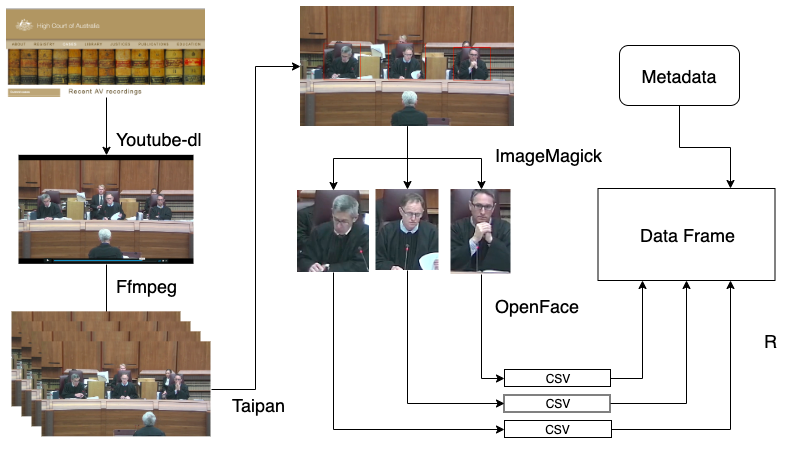
\includegraphics[width=1\linewidth]{figures/workflow} \caption{data processing workflow \label{fig:workflow}}\label{fig:unnamed-chunk-1}
\end{figure}

\hypertarget{variable-description}{%
\section{Variable description}\label{variable-description}}

OpenFace provides more than 711 variables measuring different aspect of a given face and a full description of the output variables can be found \href{https://github.com/TadasBaltrusaitis/OpenFace/wiki/Action-Units}{here}. This outlines the difficulty of this project: no existing models will present accurate prediction and inference using 700+ variables - how can we incorporate these information to say about the facial expressions of the Justices during the hearings?

I conduct some exploratory data analysis on one video: \texttt{Nauru\_a} and find the 700+ variables can be classified as follows with some insights

\begin{itemize}
\item
  \textbf{Confidence}: How confidence OpenFace is with the detection. Confidence is related to the angle that the Justice's face present in the images.
\item
  \textbf{Gaze}: Gaze tracking: the vector from the pupil to corneal reflection. The dataset contains information on the gaze for both eyes while there is no distinct difference between the eyes. Also I was trying to make animation to track the change of the gaze for judges but no good luck.
\item
  \textbf{Pose}: the location of the head with respect to camera. Pose-related variables don't provide much useful information apart from gaze-related variables.
\item
  \textbf{Landmarking}: landmarking variables for face and eyes. Landmarking variables allows me to plot the face of the judge in a particular frame. More work could be done to explore the usefulness of landmarking variables.
\item
  \textbf{Action Unit}: Action units are used to describe facial expressions. \href{https://imotions.com/blog/facial-action-coding-system/}{this website} provides a good animation on each action unit. The action unit has intensity measures ending with \texttt{\_c} and presence measures ending with \texttt{\_r}. These variables will be the focus of my project and a reference study of using action units to detect human emotion by Kovalchik can be found \href{http://www.sloansportsconference.com/wp-content/uploads/2018/02/2005.pdf}{here}.
\end{itemize}

\hypertarget{data-format}{%
\section{Data format}\label{data-format}}

In this project, we will make use of the action unit variables along with all the added indexes to analyse the face of the judge. In the wide format, apart from the first four index columns, each action unit has two columns with one for binary presence value and another for numeric intensity value. The Table \ref{tab:wide} presents the first five rows of the dataset with columns for the first action unit only.

\begin{table}[t]

\caption{\label{tab:unnamed-chunk-2}\label{tab:wide}}
\centering
\begin{tabular}{l|l|r|r|r|r|r|r|r|r|r|r|r|r|r|r|r|r|r|r|l|r|r|r|r|r|r|r|r|r|r|r|r|r|r|r|r|r|r}
\hline
judge & video & frame & AU01\_r & AU02\_r & AU04\_r & AU05\_r & AU06\_r & AU07\_r & AU09\_r & AU10\_r & AU12\_r & AU14\_r & AU15\_r & AU17\_r & AU20\_r & AU23\_r & AU25\_r & AU26\_r & AU45\_r & speaker & AU01\_c & AU02\_c & AU04\_c & AU05\_c & AU06\_c & AU07\_c & AU09\_c & AU10\_c & AU12\_c & AU14\_c & AU15\_c & AU17\_c & AU20\_c & AU23\_c & AU25\_c & AU26\_c & AU28\_c & AU45\_c\\
\hline
Bell & McKell & 1 & 0 & 0 & 0.69 & 0.63 & 0 & 1.54 & 0 & 0 & 0 & 0 & 0 & 0 & 0.05 & 0 & 0 & 0.26 & 0.47 & Appellent & 1 & 1 & 0 & 1 & 0 & 1 & 1 & 1 & 0 & 0 & 1 & 0 & 1 & 0 & 1 & 0 & 0 & 0\\
\hline
Bell & McKell & 2 & 0 & 0 & 0.69 & 0.63 & 0 & 1.54 & 0 & 0 & 0 & 0 & 0 & 0 & 0.05 & 0 & 0 & 0.26 & 0.47 & Appellent & 0 & 1 & 1 & 1 & 0 & 1 & 1 & 1 & 0 & 0 & 1 & 0 & 1 & 0 & 1 & 0 & 0 & 0\\
\hline
\end{tabular}
\end{table}

The data can also be expressed in the long format with action unit being another index and presence and intensity being two columns. The Table \ref{tab:long} presents the first five rows of the data in the long format.

\begin{table}[t]

\caption{\label{tab:unnamed-chunk-3}\label{tab:long}}
\centering
\resizebox{\linewidth}{!}{
\begin{tabular}{l|l|r|l|l|r|r}
\hline
judge & video & frame & speaker & AU & presence & intensity\\
\hline
Bell & McKell & 1 & Appellent & AU01 & 1 & 0.00\\
\hline
Bell & McKell & 1 & Appellent & AU02 & 1 & 0.00\\
\hline
Bell & McKell & 1 & Appellent & AU04 & 1 & 0.69\\
\hline
Bell & McKell & 1 & Appellent & AU05 & 0 & 0.63\\
\hline
Bell & McKell & 1 & Appellent & AU06 & 0 & 0.00\\
\hline
Bell & McKell & 1 & Appellent & AU07 & 1 & 1.54\\
\hline
Bell & McKell & 1 & Appellent & AU09 & 0 & 0.00\\
\hline
Bell & McKell & 1 & Appellent & AU10 & 0 & 0.00\\
\hline
Bell & McKell & 1 & Appellent & AU12 & 0 & 0.00\\
\hline
Bell & McKell & 1 & Appellent & AU14 & 0 & 0.00\\
\hline
Bell & McKell & 1 & Appellent & AU15 & 1 & 0.00\\
\hline
Bell & McKell & 1 & Appellent & AU17 & 0 & 0.00\\
\hline
Bell & McKell & 1 & Appellent & AU20 & 1 & 0.05\\
\hline
Bell & McKell & 1 & Appellent & AU23 & 0 & 0.00\\
\hline
Bell & McKell & 1 & Appellent & AU25 & 0 & 0.00\\
\hline
Bell & McKell & 1 & Appellent & AU26 & 0 & 0.26\\
\hline
Bell & McKell & 1 & Appellent & AU28 & NA & NA\\
\hline
Bell & McKell & 1 & Appellent & AU45 & 0 & 0.47\\
\hline
Bell & McKell & 2 & Appellent & AU01 & 0 & 0.00\\
\hline
Bell & McKell & 2 & Appellent & AU02 & 0 & 0.00\\
\hline
Bell & McKell & 2 & Appellent & AU04 & 1 & 0.69\\
\hline
Bell & McKell & 2 & Appellent & AU05 & 1 & 0.63\\
\hline
Bell & McKell & 2 & Appellent & AU06 & 1 & 0.00\\
\hline
Bell & McKell & 2 & Appellent & AU07 & 1 & 1.54\\
\hline
Bell & McKell & 2 & Appellent & AU09 & 1 & 0.00\\
\hline
Bell & McKell & 2 & Appellent & AU10 & 0 & 0.00\\
\hline
Bell & McKell & 2 & Appellent & AU12 & 0 & 0.00\\
\hline
Bell & McKell & 2 & Appellent & AU14 & 1 & 0.00\\
\hline
Bell & McKell & 2 & Appellent & AU15 & 0 & 0.00\\
\hline
Bell & McKell & 2 & Appellent & AU17 & 1 & 0.00\\
\hline
Bell & McKell & 2 & Appellent & AU20 & 1 & 0.05\\
\hline
Bell & McKell & 2 & Appellent & AU23 & 0 & 0.00\\
\hline
Bell & McKell & 2 & Appellent & AU25 & 1 & 0.00\\
\hline
Bell & McKell & 2 & Appellent & AU26 & 0 & 0.26\\
\hline
Bell & McKell & 2 & Appellent & AU28 & NA & NA\\
\hline
Bell & McKell & 2 & Appellent & AU45 & 0 & 0.47\\
\hline
\end{tabular}}
\end{table}

\hypertarget{missing-value-imputation}{%
\section{Missing value imputation}\label{missing-value-imputation}}

The missingness in the dataset could be due to the fact that a judge is reading the materials on the desk so the face is not captured for a particular frame or simply because some faces are not detectable for the given resolution of the video stream. However, since that data is in time series structure, simply drop the missing observation will cause the time interval to be irregular and complicate further analysis.

There are two different sets of variables that need imputation. \texttt{Presence} is a binary variable that takes value of one if an action unit is present in a particular frame for a judge in a video and \texttt{Intensity} measures how strong that action unit is. Linear interpolation from \texttt{forecast} package is suitable to impute \texttt{Intensity} and \texttt{Presence} is imputed through sampling from binomial distribution. The imputed action unit data is stored as \texttt{au\_imputed} under the \texttt{raw\_data} folder.

\hypertarget{data-cleaning}{%
\section{Data cleaning}\label{data-cleaning}}

There is a data quality issue coming from the data I get from OpenFace. For some observations, the intensity of the action unit could be high while the present variable has a zero value. This does not make sense since if an action unit has been detected as strong intensity for a judge in a particular frame, it should at least present on the judge's face. Therefore, I adjust for the presence value if the intensity is higher than one. One is being chosen as the threshold value since in Ekman's definition of the intensity of the action unit, a score of one means the action unit is at least slightly present in the judge's face. The adjusted data is stored as \texttt{au\_tidy} under the \texttt{raw\_data} folder.

\hypertarget{methods}{%
\chapter{Methods}\label{methods}}

Here you need to write about the analytical methods that you are using

\hypertarget{results}{%
\chapter{Results}\label{results}}

\hypertarget{notation}{%
\section{Notation}\label{notation}}

Let \(\mathbf{X}\) be a matrix of predictors, and \(\mathbf{Y}\) variable in our case is bivariate matrix of response variables, including a binary indicator of presence/absence and a numeric value measuring intensity, of facial action unit, where

\begin{itemize}
\tightlist
\item
  \(X_1\) indicates \texttt{judge} with six categories \(i = 1,2, \cdots, 6\)
\item
  \(X_2\) indicates \texttt{video} for each of the seven cases, \(j = 1,2, \cdots, 7\)
\item
  \(X_3\) indicates action unit containing 18 possible facial expression.\\
\item
  \(X_4\) indicates \texttt{speaker}, either the appellant or respondent, \(l=1,2\)
\item
  \(X_5\) indicates \texttt{frame} corresponding to time, \(t = 1,2, \cdots, T_j\)
\end{itemize}

Note that \(t\) could be considered a time variable, but because images are taken at 1 minute intervals, temporal dependence is unlikely to exist. Rather this should be considered an independent observation.

A full, main effects model for the data might be expressed as:

\[Y_{ijkl} = \mu + \alpha_i + \beta_j + \gamma_k + \delta_l + \varepsilon_{ijkl}\]

\noindent and we would be interested in interactions between judge, case, action unit and who is speaking. An alternative model structure, is to treat each action unit individually, and fit separate models.

Also, let \(P_{jitkl}\) represent the response variable presence, and \(I_{jitkl}\) represent the second response variable intensity. This notation will be helpful for defining the plots and models explained in this section.

\hypertarget{action-unit-presence}{%
\section{Action unit: Presence}\label{action-unit-presence}}

\hypertarget{mean-presence}{%
\subsection{Mean presence}\label{mean-presence}}

I first compute the average presence (\(P_{ik}\)) of each action unit for each judge as \[P_{ik} = \frac{\sum_{jt}X_{ijtk}}{\sum_{j = 1}^JT_j}\] This is then plotted in Figure \ref{fig:mean_presence} to give an overview of the presence of all the action units across all the judge. The order of action unit on the y axis is ranked by the average presence of all the judge. The five most frequent action units are highlighted in blue for each judge and summarised in Table \ref{tab:most_common}

\begin{figure}
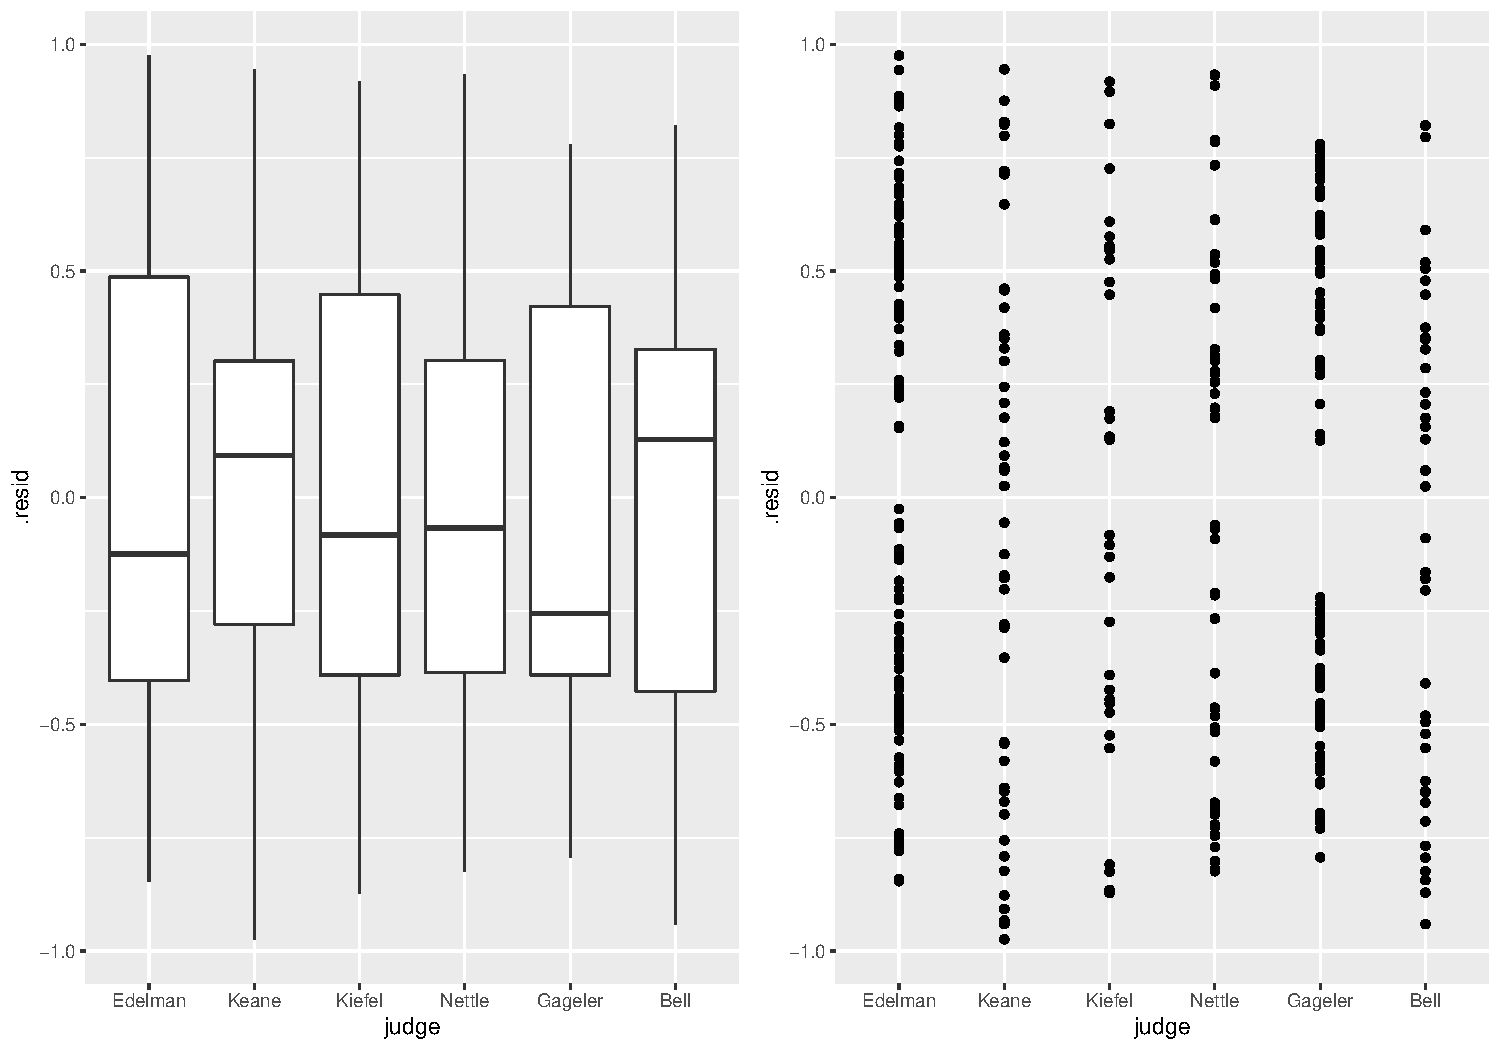
\includegraphics[width=1\linewidth]{thesis_files/figure-latex/unnamed-chunk-4-1} \caption{The average presence score of each action unit for each judge, aggregating on video and time. \label{fig:mean_presence}}\label{fig:unnamed-chunk-4}
\end{figure}

\begin{table}[t]

\caption{\label{tab:unnamed-chunk-5}\label{tab:most_common}The five most commonly presented action unit for each judge.}
\centering
\begin{tabular}{r|l|l|l|l|l|l}
\hline
index & Bell & Edelman & Gageler & Keane & Kiefel & Nettle\\
\hline
1 & AU15 & AU02 & AU02 & AU20 & AU02 & AU02\\
\hline
2 & AU25 & AU20 & AU05 & AU15 & AU25 & AU15\\
\hline
3 & AU09 & AU01 & AU14 & AU02 & AU45 & AU20\\
\hline
4 & AU02 & AU15 & AU15 & AU14 & AU20 & AU01\\
\hline
5 & AU01 & AU23 & AU20 & AU07 & AU14 & AU07\\
\hline
\end{tabular}
\end{table}

It can be seen that some of the action units are common across almost all the judges, these includes

\begin{itemize}
\tightlist
\item
  AU02 (outer eyebrow raise),
\item
  AU20 (lip stretcher),
\item
  AU15 (Lip Corner Depressor)
\item
  AU14 (Dimpler)
\end{itemize}

AU02 makes a contribution to surprise, which is a positive attitude showing that judges are interested in a particular moment {[}@ekman2002facial{]}. According to {[}@ekman2002facial{]}, AU14 indicates boredom and AU15 shows confusion. Along with other action units that presented with high frequency in a particular judge but not all (summarised in Table \ref{tab:other_highf}), the emotions judges displayed in the courtroom can be summarised into three categories, described in Table \ref{tab:three_category} along with the featured action units.

\begin{table}[t]

\caption{\label{tab:unnamed-chunk-6}\label{tab:three_category} Summarised emotions and featured action units}
\centering
\begin{tabular}{l|l}
\hline
emotion & Featured Action Unit\\
\hline
Surprise & AU01, AU02, AU05\\
\hline
Boredom & AU14, AU23\\
\hline
Confusion & AU07, AU15, AU23\\
\hline
\end{tabular}
\end{table}

\begin{table}[t]

\caption{\label{tab:unnamed-chunk-7}\label{tab:other_highf} Other high frequent action units }
\centering
\begin{tabular}{l|l|l|l}
\hline
judge\_id & first & second & third\\
\hline
Bell & AU25: Lips part & AU09: Nose wrinkler & AU01: Inner brow raiser\\
\hline
Edelman & AU01: Inner brow raiser & AU23: Lip tightener & NA\\
\hline
Gageler & AU05: Upper lid raiser & NA & NA\\
\hline
Keane & AU07: Lid tightener & NA & NA\\
\hline
Kiefel & AU25: Lips part & AU45: Blink & NA\\
\hline
Nettle & AU01: Inner brow raiser & AU07: Lid tightener & NA\\
\hline
\end{tabular}
\end{table}

\hypertarget{model-fit}{%
\subsection{Model fit}\label{model-fit}}

The first model I use is a generalised linear model with binomial link to understand the presence of the action units. The variables used include the judge, action units and their interactions. The model can be written down as Equation \ref{eq:judge_au}.Judge Edelman and AU01 are selected as the base level. Model fitting result presented in Table \ref{tab:glance_1}

\begin{equation}\label{eq:judge_au}
P_{ik} = \mu + \alpha_i + \delta_k + (\alpha\delta)_{ik}
\end{equation}

\begin{table}[t]

\caption{\label{tab:unnamed-chunk-8}\label{tab:glance_1}summary of model fit}
\centering
\begin{tabular}{r|r|r|r|r|r|r}
\hline
null.deviance & df.null & logLik & AIC & BIC & deviance & df.residual\\
\hline
35945.66 & 26571 & -14756.03 & 29596.06 & 29939.94 & 29512.06 & 26530\\
\hline
\end{tabular}
\end{table}

I'm interested to know if the presence score for one pair of judge and action unit is signficiantly different from another pair. Aanalysis of Varaince (ANOVA) test result in Table \ref{tab:anova} shows that there are significant variance for both judge, AU and their interactions. The next step after ANOVA is to test how each level of judge and AU different from another and I use multiple comparison to do this. (manually it will be 861 test to perform since 6 judges and 7 au - using multiple comparison, we can perform this take while control for a relatively low 5\% false positive rate). The estimated coefficient for each judge and AU pair is reported in Table \ref{tab:result_1} along with the upper and lower confidence interval bond. The information in the group column is helpful to understand how one particular pair of judge and au is different from another pair. With compact letter display, the pair with the same letter/number are \emph{NOT} significantly different from each other. This result is also plotted in Figure \ref{fig:result_1}.

\begin{table}[t]

\caption{\label{tab:unnamed-chunk-9}\label{tab:anova}ANOVA result}
\centering
\begin{tabular}{l|r|r|r|r}
\hline
  & Df & Deviance & Resid. Df & Resid. Dev\\
\hline
NULL & NA & NA & 26571 & 35945.66\\
\hline
judge & 5 & 192.8823 & 26566 & 35752.77\\
\hline
AU & 6 & 3051.6656 & 26560 & 32701.11\\
\hline
judge:AU & 30 & 3189.0482 & 26530 & 29512.06\\
\hline
\end{tabular}
\end{table}

\begin{table}[ht]
\begin{center}
\caption{\label{tab:result_1} model result}
\begin{tabular}{llllllll}
\toprule
judge & AU & prob & SE & df & asymp.LCL & asymp.UCL & .group \\
\midrule
Keane & AU01 & 0.12 & 0.0164 & Inf & 0.094 & 0.16 &  1                   \\
Bell & AU14 & 0.13 & 0.0170 & Inf & 0.105 & 0.17 &  1                   \\
Keane & AU25 & 0.16 & 0.0182 & Inf & 0.125 & 0.20 &  12                  \\
Nettle & AU05 & 0.24 & 0.0172 & Inf & 0.211 & 0.28 &   23                 \\
Gageler & AU01 & 0.31 & 0.0164 & Inf & 0.277 & 0.34 &    3                 \\
Edelman & AU05 & 0.31 & 0.0145 & Inf & 0.282 & 0.34 &    3                 \\
Edelman & AU25 & 0.31 & 0.0145 & Inf & 0.283 & 0.34 &    3                 \\
Kiefel & AU05 & 0.31 & 0.0196 & Inf & 0.278 & 0.35 &    34                \\
Edelman & AU14 & 0.41 & 0.0154 & Inf & 0.377 & 0.44 &     45               \\
Nettle & AU25 & 0.44 & 0.0199 & Inf & 0.399 & 0.48 &      56              \\
Edelman & AU15 & 0.44 & 0.0155 & Inf & 0.410 & 0.47 &      56              \\
Gageler & AU25 & 0.44 & 0.0176 & Inf & 0.409 & 0.48 &      56              \\
Nettle & AU14 & 0.46 & 0.0200 & Inf & 0.424 & 0.50 &      56              \\
Kiefel & AU01 & 0.50 & 0.0211 & Inf & 0.461 & 0.54 &      567             \\
Gageler & AU20 & 0.51 & 0.0177 & Inf & 0.472 & 0.54 &       67             \\
Kiefel & AU15 & 0.51 & 0.0211 & Inf & 0.468 & 0.55 &       67             \\
Kiefel & AU14 & 0.52 & 0.0211 & Inf & 0.476 & 0.56 &       678            \\
Keane & AU05 & 0.54 & 0.0249 & Inf & 0.490 & 0.59 &       6789           \\
Bell & AU05 & 0.55 & 0.0249 & Inf & 0.497 & 0.59 &       6789           \\
Edelman & AU01 & 0.59 & 0.0154 & Inf & 0.559 & 0.62 &        7890          \\
Gageler & AU15 & 0.62 & 0.0172 & Inf & 0.588 & 0.66 &         890A         \\
Gageler & AU14 & 0.63 & 0.0172 & Inf & 0.592 & 0.66 &          90A         \\
Gageler & AU05 & 0.67 & 0.0166 & Inf & 0.640 & 0.71 &           0AB        \\
Bell & AU20 & 0.68 & 0.0232 & Inf & 0.636 & 0.73 &           0AB        \\
Bell & AU01 & 0.69 & 0.0232 & Inf & 0.639 & 0.73 &           0AB        \\
Nettle & AU01 & 0.69 & 0.0186 & Inf & 0.653 & 0.73 &            AB        \\
Keane & AU14 & 0.72 & 0.0225 & Inf & 0.672 & 0.76 &            AB        \\
Nettle & AU20 & 0.75 & 0.0174 & Inf & 0.713 & 0.78 &             BC       \\
Bell & AU02 & 0.75 & 0.0216 & Inf & 0.706 & 0.79 &             BCD      \\
Edelman & AU20 & 0.75 & 0.0135 & Inf & 0.725 & 0.78 &             BC       \\
Nettle & AU15 & 0.75 & 0.0173 & Inf & 0.719 & 0.79 &             BCD      \\
Keane & AU02 & 0.78 & 0.0207 & Inf & 0.737 & 0.82 &             BCDE     \\
Bell & AU25 & 0.84 & 0.0183 & Inf & 0.801 & 0.87 &              CDEF    \\
Bell & AU15 & 0.85 & 0.0177 & Inf & 0.815 & 0.88 &               DEF    \\
Kiefel & AU20 & 0.85 & 0.0150 & Inf & 0.821 & 0.88 &                EF    \\
Gageler & AU02 & 0.86 & 0.0123 & Inf & 0.836 & 0.88 &                EF    \\
Keane & AU15 & 0.88 & 0.0164 & Inf & 0.842 & 0.91 &                EF    \\
Kiefel & AU25 & 0.89 & 0.0135 & Inf & 0.856 & 0.91 &                 FG   \\
Keane & AU20 & 0.92 & 0.0135 & Inf & 0.889 & 0.94 &                 FGH  \\
Edelman & AU02 & 0.94 & 0.0074 & Inf & 0.925 & 0.95 &                  GH  \\
Kiefel & AU02 & 0.96 & 0.0087 & Inf & 0.935 & 0.97 &                   HI \\
Nettle & AU02 & 1.00 & 0.0028 & Inf & 0.985 & 1.00 &                    I \\
\bottomrule
\end{tabular}
\end{center}
\end{table}

\begin{figure}
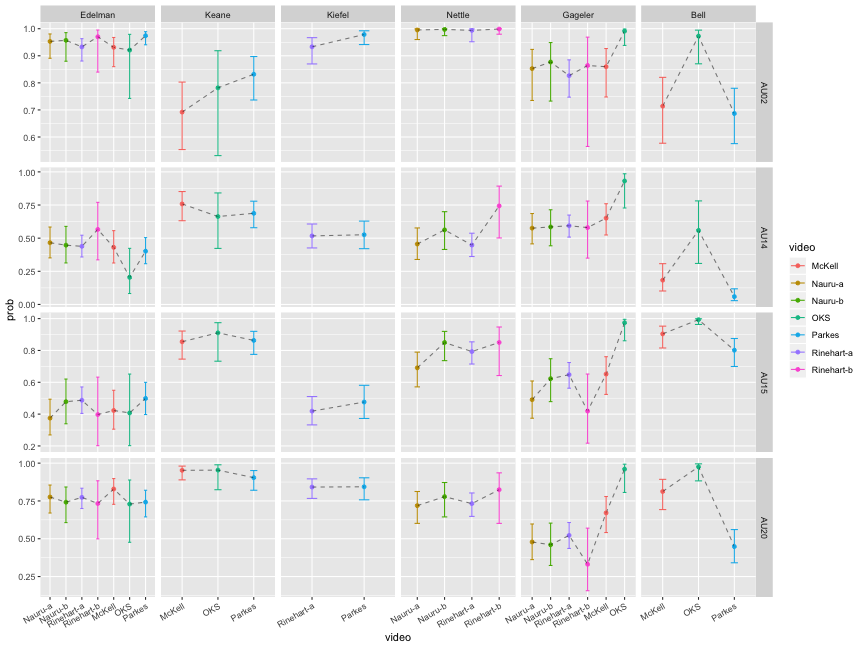
\includegraphics[width=1\linewidth]{thesis_files/figure-latex/unnamed-chunk-10-1} \caption{plot the multiple comparison result \label{fig:result_1}}\label{fig:unnamed-chunk-10}
\end{figure}

\hypertarget{presence-by-videos}{%
\subsection{Presence by videos}\label{presence-by-videos}}

Apart from visualising the general presence score for all the action unit, I'm also interested in the break down statistics by video (\(P_{ijk}\)). This is computed as \[P_{ijk} = \frac{\sum_{t}X_{ijtk}}{T_j}\] for the four most common action units: AU02, AU14, AU15, AU20 and plotted in Figure \ref{fig:common_video}. From this plot, we can observe that some of the judge are have relatively stable display of action unit throughout different videos (i.e.~Edelman and Nettle), while Gagaler seems to be highly reactive to some cases (i.e.~OKS).

\begin{figure}
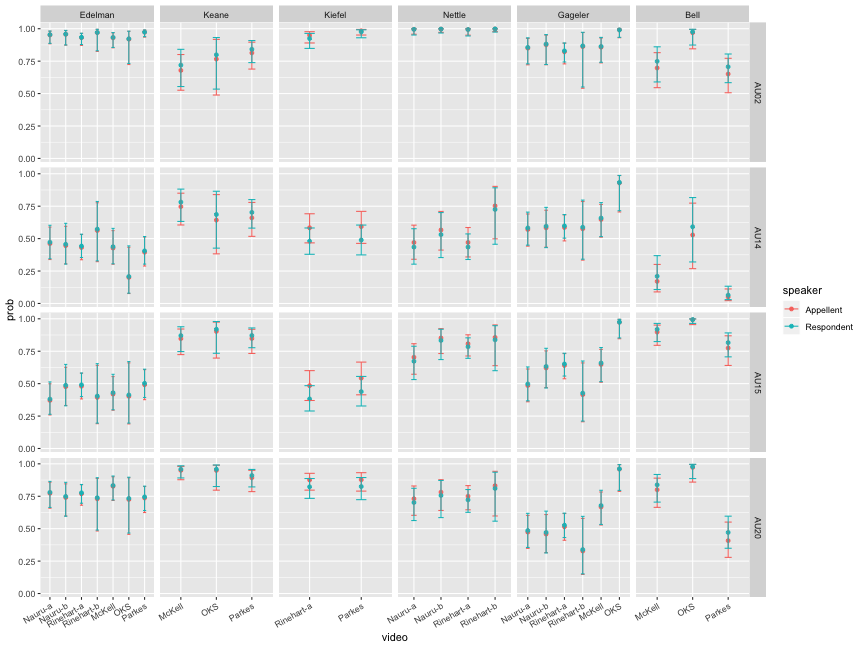
\includegraphics[width=1\linewidth]{thesis_files/figure-latex/unnamed-chunk-11-1} \caption{Average presence of the four most common action units for each judge by video\label{fig:common_video}}\label{fig:unnamed-chunk-11}
\end{figure}

\hypertarget{model-fit-1}{%
\subsection{Model fit}\label{model-fit-1}}

\begin{equation}\label{eq:judge_au_video}
P_{ijk} = \mu + \alpha_i + \beta_j +\delta_k + (\alpha\beta)_{ij}+(\alpha\delta)_{ik} + (\beta\delta)_{jk}
\end{equation}

\hypertarget{appellant-vs.respondent}{%
\subsection{Appellant vs.~Respondent}\label{appellant-vs.respondent}}

\begin{table}[t]

\caption{\label{tab:unnamed-chunk-15}\label{tab:glance_3}summary of model fit}
\centering
\begin{tabular}{r|r|r|r|r|r|r}
\hline
null.deviance & df.null & logLik & AIC & BIC & deviance & df.residual\\
\hline
35945.66 & 26571 & -14609.05 & 29388.1 & 30084.05 & 29218.1 & 26487\\
\hline
\end{tabular}
\end{table}

\hypertarget{action-unit-intensity}{%
\section{Action unit: Intensity}\label{action-unit-intensity}}

\hypertarget{general-intensity-plot}{%
\subsection{General Intensity plot}\label{general-intensity-plot}}

In Ekman's 20002 FACS manual, the intensity of an action unit is defined based on five classes: Trace: 0-1, Slight: 1-2, Marked or pronounced: 2-3, Severe or extreme: 3-4 and Maximum: 4-5.

The boxplot of the intensity for all the judges across all the videos is presented in Figure \ref{fig:intensity}. Each bar-and-whisker represents the intensity (\(I_{ijtk}\)) of all the action units aggregated on time for a particular judge \(i\) in a specific case \(j\). For example, the first bar-and-whisker in case Nauru\_a is created using all the 17 action units of Edelman through out the elapsed time in Nauru\_a case.

From the plot, we can see that most of the action units have low intensity score and this is expected because usually judges are expected to behave neutral in the court room. Thus a square root transformation is taken on the y axis for better visualisation effect. We can find that Judge Nettle seems to have higher average in all the four cases he appears: Nauru\_a\&b, Rinehart\_a \&b.

\begin{figure}
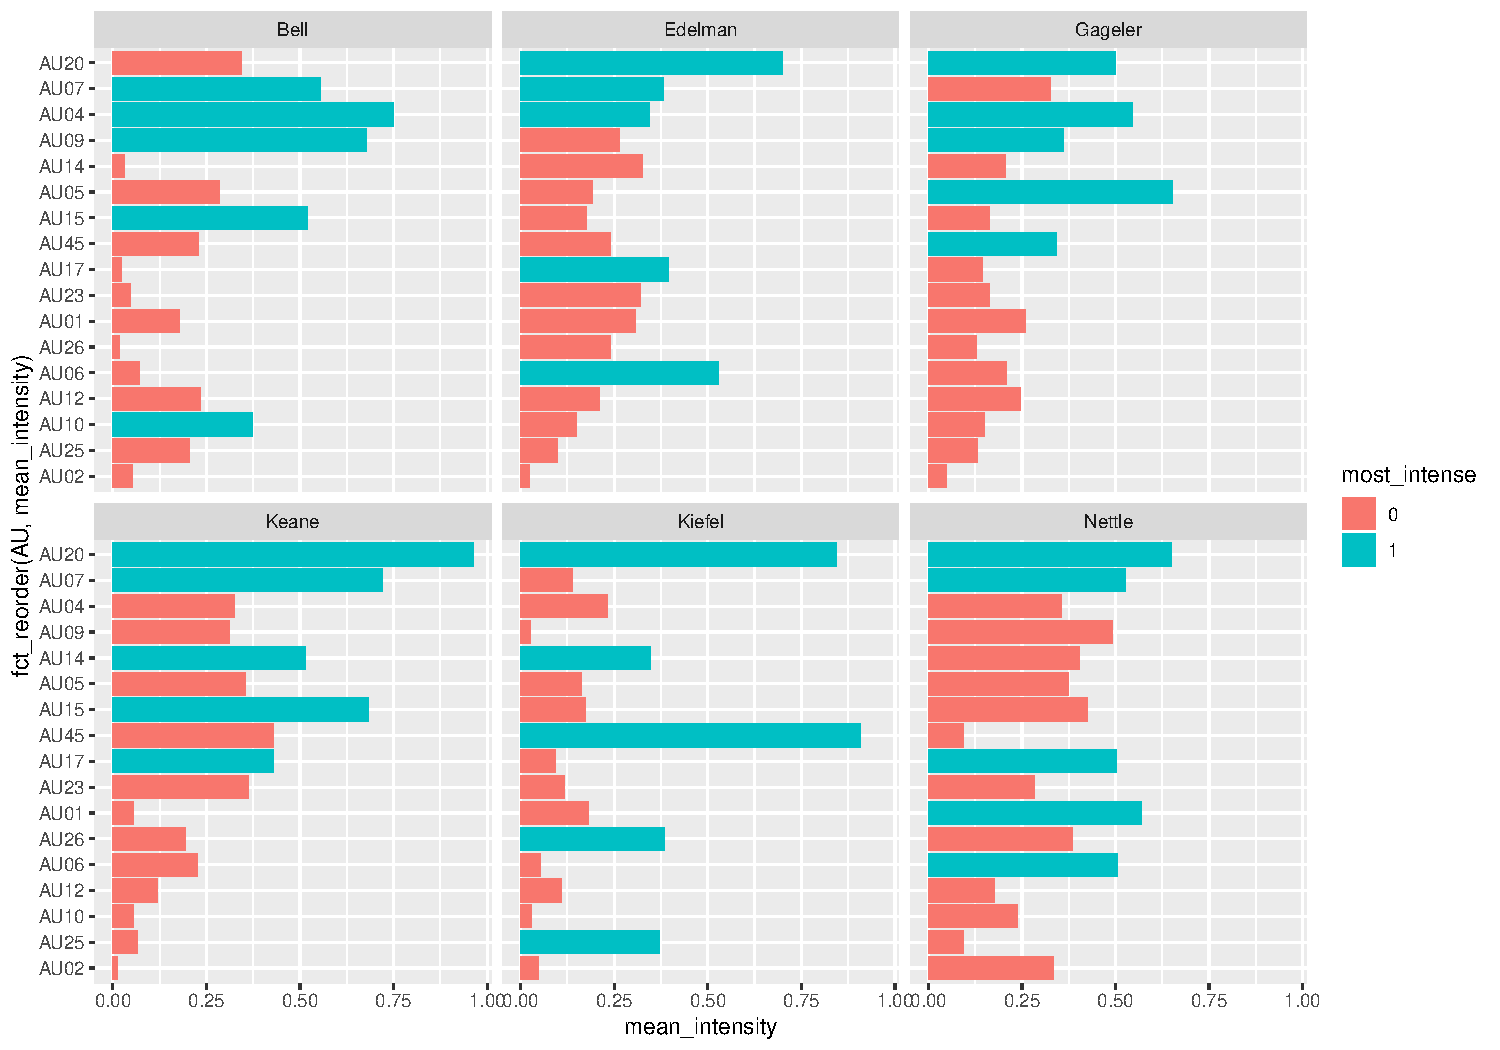
\includegraphics[width=1\linewidth]{thesis_files/figure-latex/unnamed-chunk-16-1} \caption{General intensity score by judge and video\label{fig:intensity}}\label{fig:unnamed-chunk-16}
\end{figure}

\hypertarget{mean-intensity}{%
\subsection{Mean intensity}\label{mean-intensity}}

Mean intensity score (\(I_{ik}\)) of each action unit for each of the judge is computed as \[I_{ik} = \frac{\sum_{jt}X_{ijtk}}{\sum_{j = 1}^JT_j}\] and plotted in Figure \ref{fig:mean_intensity}. The five most intense action units for each judge are presented in Table \ref{tab:most_intense}. We can find that the common high intense action units includes

\begin{itemize}
\tightlist
\item
  AU20 (Lip Stretcher)
\item
  AU07 (Lid Tightener)
\item
  AU04 (Brow Lowerer)
\end{itemize}

AU04 also belongs to the confusion category as AU07. This could help to understand that judges are more likely to express a stronger confusing expression than other emotions.

\begin{figure}
\includegraphics[width=1\linewidth]{thesis_files/figure-latex/unnamed-chunk-18-1} \caption{Mean intensity score for each judge and action unit aggregating on videos.\label{fig:mean_intensity}}\label{fig:unnamed-chunk-18}
\end{figure}

\begin{table}[t]

\caption{\label{tab:unnamed-chunk-19}\label{tab:most_intense}The five most intense action unit for each judge.}
\centering
\begin{tabular}{r|l|l|l|l|l|l}
\hline
index & Bell & Edelman & Gageler & Keane & Kiefel & Nettle\\
\hline
1 & AU04 & AU20 & AU05 & AU20 & AU45 & AU20\\
\hline
2 & AU09 & AU06 & AU04 & AU07 & AU20 & AU01\\
\hline
3 & AU07 & AU17 & AU20 & AU15 & AU26 & AU07\\
\hline
4 & AU15 & AU07 & AU09 & AU14 & AU25 & AU06\\
\hline
5 & AU10 & AU04 & AU45 & AU17 & AU14 & AU17\\
\hline
\end{tabular}
\end{table}

\hypertarget{intensity-plot-for-the-most-frequent-action-units}{%
\subsection{Intensity plot for the most frequent action units}\label{intensity-plot-for-the-most-frequent-action-units}}

Apart from visualising the general intensity score for all the action units, I'm also interested in the intensity score of the most frequent action units. Figure \ref{fig:intensity_by_au} presents this. The statistics being plotted is \(I_{ijtk}\) with \(k\) including AU02, AU14, AU15 and AU20 as the most common four action units. From this plot, we can learn that AU02, although being commonly detected for all the judges, has low intensity score.

\begin{figure}
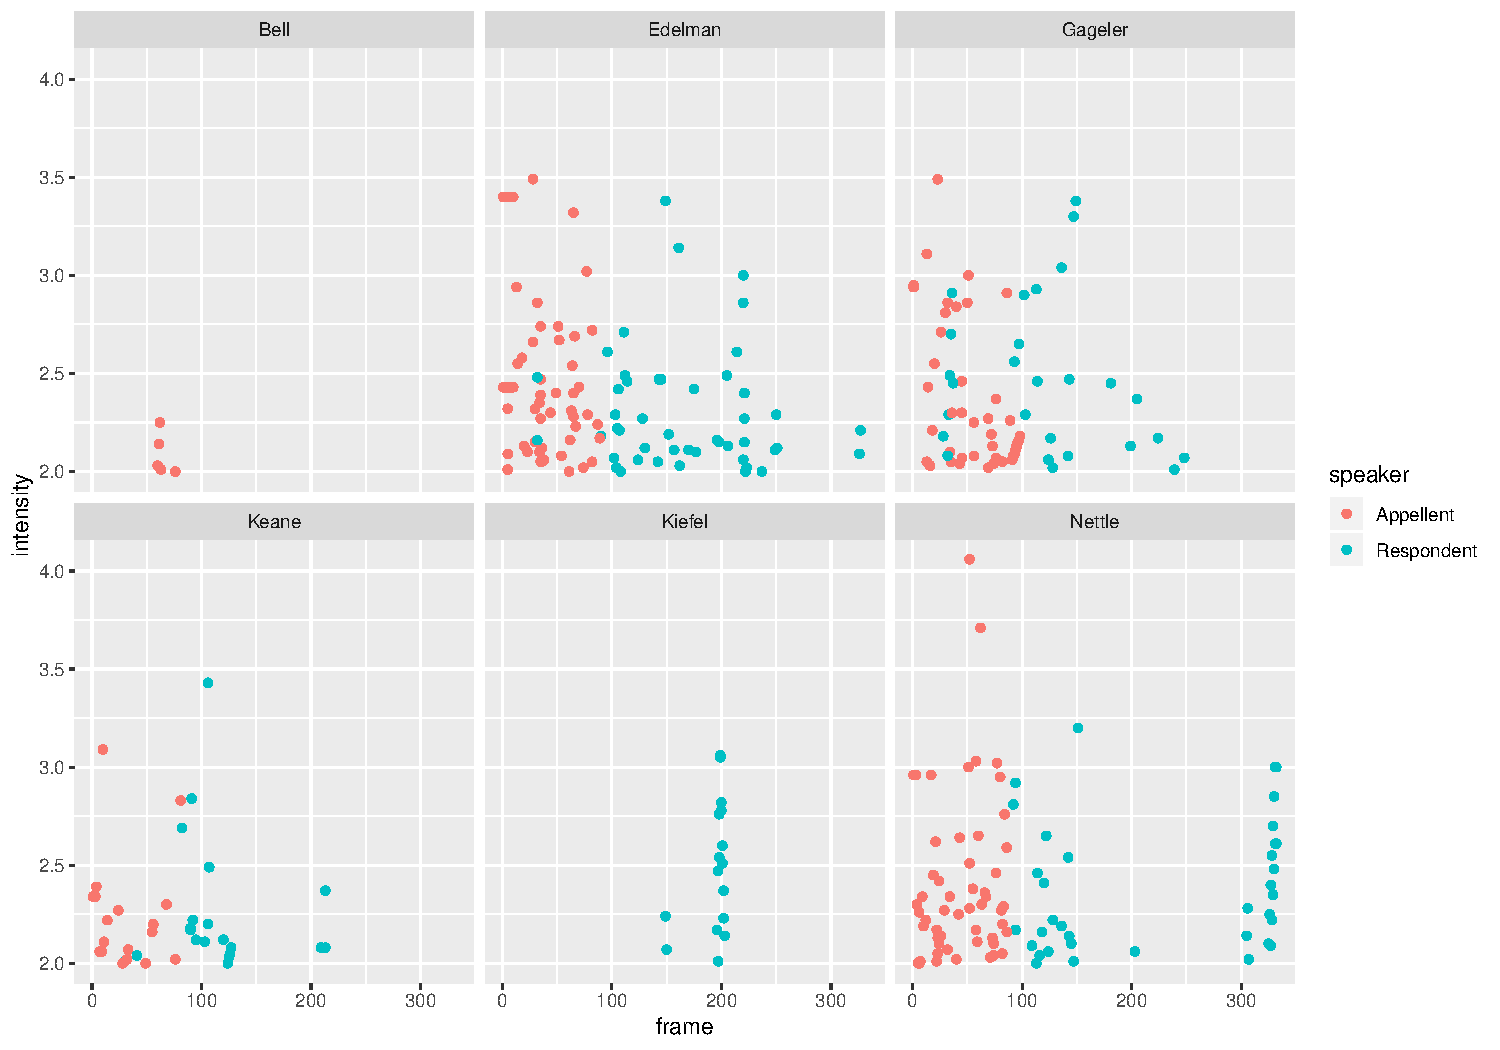
\includegraphics[width=1\linewidth]{thesis_files/figure-latex/unnamed-chunk-20-1} \caption{Intensity score of the most frequent action units, seperating by judge and video ID.\label{fig:intensity_by_au}}\label{fig:unnamed-chunk-20}
\end{figure}

\hypertarget{high-intensity-points}{%
\subsection{High intensity points}\label{high-intensity-points}}

We filter out the points have intensity greater than 2 (at least ``slight'' as per Ekman) in the previous plot and plot it against time and color by the speaker. It tells us that Edelman, Gageler and Nettle are the judges have stronger emotion that can be detected (since they have more points with intensity greater than 2). Different judges also have different time where they display stronger emotions. For example, Justice Nettle are more likely to have stronger emotion throughout the time when the appellant is speaking but only at the beginning and ending period when the respondent is speaking.

\includegraphics[width=1\linewidth]{thesis_files/figure-latex/unnamed-chunk-21-1}

\appendix

\hypertarget{additional-stuff}{%
\chapter{Additional stuff}\label{additional-stuff}}

\begin{longtable}[]{@{}lll@{}}
\caption{Details of videos processed.}\tabularnewline
\toprule
\begin{minipage}[b]{0.42\columnwidth}\raggedright
Case\strut
\end{minipage} & \begin{minipage}[b]{0.14\columnwidth}\raggedright
Name\strut
\end{minipage} & \begin{minipage}[b]{0.35\columnwidth}\raggedright
AV recording link\strut
\end{minipage}\tabularnewline
\midrule
\endfirsthead
\toprule
\begin{minipage}[b]{0.42\columnwidth}\raggedright
Case\strut
\end{minipage} & \begin{minipage}[b]{0.14\columnwidth}\raggedright
Name\strut
\end{minipage} & \begin{minipage}[b]{0.35\columnwidth}\raggedright
AV recording link\strut
\end{minipage}\tabularnewline
\midrule
\endhead
\begin{minipage}[t]{0.42\columnwidth}\raggedright
Republic of Nauru v. WET040\strut
\end{minipage} & \begin{minipage}[t]{0.14\columnwidth}\raggedright
\texttt{Nauru\_a}\strut
\end{minipage} & \begin{minipage}[t]{0.35\columnwidth}\raggedright
\url{http://www.hcourt.gov.au/cases/cases-av/av-2018-11-07a}\strut
\end{minipage}\tabularnewline
\begin{minipage}[t]{0.42\columnwidth}\raggedright
TTY167 v. Republic of Nauru\strut
\end{minipage} & \begin{minipage}[t]{0.14\columnwidth}\raggedright
\texttt{Nauru\_b}\strut
\end{minipage} & \begin{minipage}[t]{0.35\columnwidth}\raggedright
\url{http://www.hcourt.gov.au/cases/cases-av/av-2018-11-07b}\strut
\end{minipage}\tabularnewline
\begin{minipage}[t]{0.42\columnwidth}\raggedright
Rinehart \& Anor v. Hancock Prospecting Pty Ltd \& Ors on 13 Nov 18\strut
\end{minipage} & \begin{minipage}[t]{0.14\columnwidth}\raggedright
\texttt{Rinehart\_a}\strut
\end{minipage} & \begin{minipage}[t]{0.35\columnwidth}\raggedright
\url{http://www.hcourt.gov.au/cases/cases-av/av-2018-11-13}\strut
\end{minipage}\tabularnewline
\begin{minipage}[t]{0.42\columnwidth}\raggedright
Rinehart \& Anor v. Hancock Prospecting Pty Ltd \& Ors on 14 Nov 18\strut
\end{minipage} & \begin{minipage}[t]{0.14\columnwidth}\raggedright
\texttt{Rinehart\_b}\strut
\end{minipage} & \begin{minipage}[t]{0.35\columnwidth}\raggedright
\url{http://www.hcourt.gov.au/cases/cases-av/av-2018-11-14a}\strut
\end{minipage}\tabularnewline
\begin{minipage}[t]{0.42\columnwidth}\raggedright
Parkes Shire Council v. South West Helicopters Pty Limited\strut
\end{minipage} & \begin{minipage}[t]{0.14\columnwidth}\raggedright
\texttt{Parkes}\strut
\end{minipage} & \begin{minipage}[t]{0.35\columnwidth}\raggedright
\url{http://www.hcourt.gov.au/cases/cases-av/av-2018-11-14b}\strut
\end{minipage}\tabularnewline
\begin{minipage}[t]{0.42\columnwidth}\raggedright
McKell v. The Queen\strut
\end{minipage} & \begin{minipage}[t]{0.14\columnwidth}\raggedright
\texttt{McKell}\strut
\end{minipage} & \begin{minipage}[t]{0.35\columnwidth}\raggedright
\url{http://www.hcourt.gov.au/cases/cases-av/av-2018-12-07}\strut
\end{minipage}\tabularnewline
\begin{minipage}[t]{0.42\columnwidth}\raggedright
OKS v. The State of Western Australia\strut
\end{minipage} & \begin{minipage}[t]{0.14\columnwidth}\raggedright
\texttt{OKS}\strut
\end{minipage} & \begin{minipage}[t]{0.35\columnwidth}\raggedright
\url{http://www.hcourt.gov.au/cases/cases-av/av-2019-02-14}\strut
\end{minipage}\tabularnewline
\bottomrule
\end{longtable}

\hypertarget{list-of-the-name-of-ction-units}{%
\section{List of the name of ction units}\label{list-of-the-name-of-ction-units}}

\begin{tabular}{l}
\hline
AU\_meaning\\
\hline
AU01: Inner brow raiser\\
\hline
AU02: Outer brow raiser\\
\hline
AU04: Brow lowerer\\
\hline
AU05: Upper lid raiser\\
\hline
AU06: Cheek raiser\\
\hline
AU07: Lid tightener\\
\hline
AU09: Nose wrinkler\\
\hline
AU10: Upper lip raiser\\
\hline
AU12: Lip corner puller\\
\hline
AU14: Dimpler\\
\hline
AU15: Lip corner depressor\\
\hline
AU17: Chin raiser\\
\hline
AU20: Lip stretcher\\
\hline
AU23: Lip tightener\\
\hline
AU25: Lips part\\
\hline
AU26: Jaw drop\\
\hline
AU28: Lip suck\\
\hline
AU45: Blink\\
\hline
\end{tabular}

\hypertarget{model-results}{%
\section{Model results}\label{model-results}}

\begin{tabular}{l|r|r|r|r}
\hline
term & estimate & std.error & statistic & p.value\\
\hline
(Intercept) & 0.36 & 0.06 & 5.70 & 0.00\\
\hline
judgeBell & 0.42 & 0.12 & 3.35 & 0.00\\
\hline
judgeGageler & -1.17 & 0.10 & -11.72 & 0.00\\
\hline
judgeKeane & -2.33 & 0.17 & -14.13 & 0.00\\
\hline
judgeKiefel & -0.35 & 0.11 & -3.32 & 0.00\\
\hline
judgeNettle & 0.44 & 0.11 & 4.08 & 0.00\\
\hline
AUAU02 & 2.41 & 0.15 & 16.35 & 0.00\\
\hline
AUAU05 & -1.16 & 0.09 & -12.54 & 0.00\\
\hline
AUAU14 & -0.74 & 0.09 & -8.23 & 0.00\\
\hline
AUAU15 & -0.60 & 0.09 & -6.75 & 0.00\\
\hline
AUAU20 & 0.75 & 0.10 & 7.76 & 0.00\\
\hline
AUAU25 & -1.16 & 0.09 & -12.49 & 0.00\\
\hline
judgeBell:AUAU02 & -2.09 & 0.22 & -9.68 & 0.00\\
\hline
judgeGageler:AUAU02 & 0.22 & 0.20 & 1.14 & 0.25\\
\hline
judgeKeane:AUAU02 & 0.83 & 0.24 & 3.40 & 0.00\\
\hline
judgeKiefel:AUAU02 & 0.64 & 0.27 & 2.40 & 0.02\\
\hline
judgeNettle:AUAU02 & 2.11 & 0.60 & 3.50 & 0.00\\
\hline
judgeBell:AUAU05 & 0.57 & 0.17 & 3.27 & 0.00\\
\hline
judgeGageler:AUAU05 & 2.70 & 0.14 & 18.95 & 0.00\\
\hline
judgeKeane:AUAU05 & 3.29 & 0.20 & 16.08 & 0.00\\
\hline
judgeKiefel:AUAU05 & 0.38 & 0.16 & 2.43 & 0.02\\
\hline
judgeNettle:AUAU05 & -0.77 & 0.16 & -4.88 & 0.00\\
\hline
judgeBell:AUAU14 & -1.90 & 0.20 & -9.37 & 0.00\\
\hline
judgeGageler:AUAU14 & 2.06 & 0.14 & 14.81 & 0.00\\
\hline
judgeKeane:AUAU14 & 3.65 & 0.21 & 17.46 & 0.00\\
\hline
judgeKiefel:AUAU14 & 0.80 & 0.15 & 5.33 & 0.00\\
\hline
judgeNettle:AUAU14 & -0.21 & 0.15 & -1.41 & 0.16\\
\hline
judgeBell:AUAU15 & 1.58 & 0.20 & 7.96 & 0.00\\
\hline
judgeGageler:AUAU15 & 1.91 & 0.14 & 13.75 & 0.00\\
\hline
judgeKeane:AUAU15 & 4.55 & 0.23 & 19.48 & 0.00\\
\hline
judgeKiefel:AUAU15 & 0.63 & 0.15 & 4.24 & 0.00\\
\hline
judgeNettle:AUAU15 & 0.93 & 0.16 & 5.95 & 0.00\\
\hline
judgeBell:AUAU20 & -0.76 & 0.18 & -4.22 & 0.00\\
\hline
judgeGageler:AUAU20 & 0.08 & 0.14 & 0.59 & 0.55\\
\hline
judgeKeane:AUAU20 & 3.67 & 0.26 & 14.23 & 0.00\\
\hline
judgeKiefel:AUAU20 & 1.00 & 0.18 & 5.71 & 0.00\\
\hline
judgeNettle:AUAU20 & -0.46 & 0.16 & -2.88 & 0.00\\
\hline
judgeBell:AUAU25 & 2.04 & 0.20 & 10.36 & 0.00\\
\hline
judgeGageler:AUAU25 & 1.74 & 0.14 & 12.42 & 0.00\\
\hline
judgeKeane:AUAU25 & 1.45 & 0.23 & 6.45 & 0.00\\
\hline
judgeKiefel:AUAU25 & 3.20 & 0.18 & 17.48 & 0.00\\
\hline
judgeNettle:AUAU25 & 0.11 & 0.15 & 0.70 & 0.48\\
\hline
\end{tabular}

\begin{tabular}{l|r|r|r|r}
\hline
term & estimate & std.error & statistic & p.value\\
\hline
(Intercept) & 0.64 & 0.12 & 5.47 & 0.00\\
\hline
judgeBell & 0.63 & 0.14 & 4.56 & 0.00\\
\hline
judgeGageler & -1.22 & 0.10 & -11.73 & 0.00\\
\hline
judgeKeane & -2.20 & 0.18 & -12.45 & 0.00\\
\hline
judgeKiefel & -0.38 & 0.11 & -3.43 & 0.00\\
\hline
judgeNettle & 0.31 & 0.11 & 2.71 & 0.01\\
\hline
AUAU02 & 2.11 & 0.25 & 8.31 & 0.00\\
\hline
AUAU05 & -1.51 & 0.17 & -8.96 & 0.00\\
\hline
AUAU14 & -1.02 & 0.16 & -6.30 & 0.00\\
\hline
AUAU15 & -1.35 & 0.16 & -8.19 & 0.00\\
\hline
AUAU20 & 0.36 & 0.17 & 2.11 & 0.03\\
\hline
AUAU25 & -1.11 & 0.16 & -6.83 & 0.00\\
\hline
videoNauru\_b & -0.30 & 0.16 & -1.91 & 0.06\\
\hline
videoMcKell & -0.93 & 0.16 & -5.89 & 0.00\\
\hline
videoOKS & 0.32 & 0.21 & 1.51 & 0.13\\
\hline
videoParkes & -0.34 & 0.14 & -2.38 & 0.02\\
\hline
videoRinehart\_a & -0.18 & 0.12 & -1.50 & 0.13\\
\hline
videoRinehart\_b & -0.02 & 0.23 & -0.09 & 0.93\\
\hline
judgeBell:AUAU02 & -2.42 & 0.25 & -9.63 & 0.00\\
\hline
judgeGageler:AUAU02 & 0.33 & 0.20 & 1.67 & 0.09\\
\hline
judgeKeane:AUAU02 & 0.59 & 0.28 & 2.13 & 0.03\\
\hline
judgeKiefel:AUAU02 & 0.66 & 0.28 & 2.41 & 0.02\\
\hline
judgeNettle:AUAU02 & 2.30 & 0.61 & 3.79 & 0.00\\
\hline
judgeBell:AUAU05 & 0.47 & 0.19 & 2.43 & 0.02\\
\hline
judgeGageler:AUAU05 & 2.74 & 0.15 & 18.57 & 0.00\\
\hline
judgeKeane:AUAU05 & 3.27 & 0.22 & 14.68 & 0.00\\
\hline
judgeKiefel:AUAU05 & 0.34 & 0.16 & 2.08 & 0.04\\
\hline
judgeNettle:AUAU05 & -0.70 & 0.17 & -4.22 & 0.00\\
\hline
judgeBell:AUAU14 & -2.15 & 0.22 & -9.81 & 0.00\\
\hline
judgeGageler:AUAU14 & 2.08 & 0.14 & 14.47 & 0.00\\
\hline
judgeKeane:AUAU14 & 3.50 & 0.23 & 15.54 & 0.00\\
\hline
judgeKiefel:AUAU14 & 0.93 & 0.16 & 5.89 & 0.00\\
\hline
judgeNettle:AUAU14 & -0.07 & 0.16 & -0.41 & 0.68\\
\hline
judgeBell:AUAU15 & 1.19 & 0.22 & 5.49 & 0.00\\
\hline
judgeGageler:AUAU15 & 2.02 & 0.14 & 13.93 & 0.00\\
\hline
judgeKeane:AUAU15 & 4.23 & 0.25 & 17.03 & 0.00\\
\hline
judgeKiefel:AUAU15 & 0.67 & 0.16 & 4.25 & 0.00\\
\hline
judgeNettle:AUAU15 & 1.21 & 0.17 & 7.32 & 0.00\\
\hline
judgeBell:AUAU20 & -1.18 & 0.20 & -5.78 & 0.00\\
\hline
judgeGageler:AUAU20 & 0.07 & 0.15 & 0.47 & 0.64\\
\hline
judgeKeane:AUAU20 & 3.37 & 0.28 & 12.23 & 0.00\\
\hline
judgeKiefel:AUAU20 & 1.15 & 0.18 & 6.28 & 0.00\\
\hline
judgeNettle:AUAU20 & -0.22 & 0.17 & -1.30 & 0.19\\
\hline
judgeBell:AUAU25 & 2.12 & 0.22 & 9.75 & 0.00\\
\hline
judgeGageler:AUAU25 & 1.73 & 0.15 & 11.91 & 0.00\\
\hline
judgeKeane:AUAU25 & 1.60 & 0.24 & 6.58 & 0.00\\
\hline
judgeKiefel:AUAU25 & 3.32 & 0.19 & 17.40 & 0.00\\
\hline
judgeNettle:AUAU25 & 0.07 & 0.16 & 0.43 & 0.67\\
\hline
AUAU02:videoNauru\_b & 0.48 & 0.36 & 1.36 & 0.17\\
\hline
AUAU05:videoNauru\_b & 0.18 & 0.23 & 0.78 & 0.44\\
\hline
AUAU14:videoNauru\_b & 0.44 & 0.22 & 2.03 & 0.04\\
\hline
AUAU15:videoNauru\_b & 0.91 & 0.22 & 4.08 & 0.00\\
\hline
AUAU20:videoNauru\_b & 0.36 & 0.23 & 1.61 & 0.11\\
\hline
AUAU25:videoNauru\_b & 0.20 & 0.22 & 0.91 & 0.36\\
\hline
AUAU02:videoMcKell & 0.72 & 0.30 & 2.42 & 0.02\\
\hline
AUAU05:videoMcKell & 1.13 & 0.22 & 5.15 & 0.00\\
\hline
AUAU14:videoMcKell & 1.01 & 0.22 & 4.69 & 0.00\\
\hline
AUAU15:videoMcKell & 1.45 & 0.22 & 6.63 & 0.00\\
\hline
AUAU20:videoMcKell & 1.58 & 0.23 & 6.98 & 0.00\\
\hline
AUAU25:videoMcKell & 0.20 & 0.22 & 0.88 & 0.38\\
\hline
AUAU02:videoOKS & 0.23 & 0.40 & 0.58 & 0.56\\
\hline
AUAU05:videoOKS & -1.21 & 0.30 & -4.05 & 0.00\\
\hline
AUAU14:videoOKS & 0.21 & 0.30 & 0.71 & 0.48\\
\hline
AUAU15:videoOKS & 1.37 & 0.34 & 4.06 & 0.00\\
\hline
AUAU20:videoOKS & 1.06 & 0.34 & 3.08 & 0.00\\
\hline
AUAU25:videoOKS & -0.85 & 0.30 & -2.81 & 0.00\\
\hline
AUAU02:videoParkes & 0.63 & 0.30 & 2.07 & 0.04\\
\hline
AUAU05:videoParkes & 0.30 & 0.21 & 1.45 & 0.15\\
\hline
AUAU14:videoParkes & 0.23 & 0.20 & 1.16 & 0.25\\
\hline
AUAU15:videoParkes & 0.94 & 0.20 & 4.58 & 0.00\\
\hline
AUAU20:videoParkes & 0.34 & 0.21 & 1.57 & 0.12\\
\hline
AUAU25:videoParkes & -0.21 & 0.21 & -1.02 & 0.31\\
\hline
AUAU02:videoRinehart\_a & 0.07 & 0.26 & 0.25 & 0.80\\
\hline
AUAU05:videoRinehart\_a & 0.43 & 0.17 & 2.51 & 0.01\\
\hline
AUAU14:videoRinehart\_a & 0.09 & 0.16 & 0.53 & 0.59\\
\hline
AUAU15:videoRinehart\_a & 0.55 & 0.17 & 3.28 & 0.00\\
\hline
AUAU20:videoRinehart\_a & 0.18 & 0.17 & 1.08 & 0.28\\
\hline
AUAU25:videoRinehart\_a & -0.13 & 0.17 & -0.80 & 0.42\\
\hline
AUAU02:videoRinehart\_b & 0.04 & 0.50 & 0.09 & 0.93\\
\hline
AUAU05:videoRinehart\_b & 0.19 & 0.33 & 0.58 & 0.56\\
\hline
AUAU14:videoRinehart\_b & 0.26 & 0.32 & 0.83 & 0.40\\
\hline
AUAU15:videoRinehart\_b & 0.49 & 0.32 & 1.53 & 0.13\\
\hline
AUAU20:videoRinehart\_b & -0.15 & 0.32 & -0.45 & 0.65\\
\hline
AUAU25:videoRinehart\_b & 0.42 & 0.31 & 1.33 & 0.18\\
\hline
\end{tabular}

\begin{tabular}{l|r|r|r|r}
\hline
term & estimate & std.error & statistic & p.value\\
\hline
(Intercept) & 0.64 & 0.12 & 5.43 & 0.00\\
\hline
judgeBell & 0.63 & 0.14 & 4.56 & 0.00\\
\hline
judgeGageler & -1.22 & 0.10 & -11.73 & 0.00\\
\hline
judgeKeane & -2.20 & 0.18 & -12.45 & 0.00\\
\hline
judgeKiefel & -0.38 & 0.11 & -3.43 & 0.00\\
\hline
judgeNettle & 0.31 & 0.11 & 2.71 & 0.01\\
\hline
AUAU02 & 2.11 & 0.25 & 8.31 & 0.00\\
\hline
AUAU05 & -1.51 & 0.17 & -8.96 & 0.00\\
\hline
AUAU14 & -1.02 & 0.16 & -6.30 & 0.00\\
\hline
AUAU15 & -1.35 & 0.16 & -8.19 & 0.00\\
\hline
AUAU20 & 0.36 & 0.17 & 2.11 & 0.03\\
\hline
AUAU25 & -1.11 & 0.16 & -6.83 & 0.00\\
\hline
videoNauru\_b & -0.30 & 0.16 & -1.90 & 0.06\\
\hline
videoMcKell & -0.93 & 0.16 & -5.89 & 0.00\\
\hline
videoOKS & 0.32 & 0.21 & 1.51 & 0.13\\
\hline
videoParkes & -0.34 & 0.14 & -2.38 & 0.02\\
\hline
videoRinehart\_a & -0.18 & 0.12 & -1.50 & 0.13\\
\hline
videoRinehart\_b & -0.02 & 0.23 & -0.08 & 0.93\\
\hline
speakerRespondent & 0.00 & 0.03 & 0.06 & 0.95\\
\hline
judgeBell:AUAU02 & -2.42 & 0.25 & -9.63 & 0.00\\
\hline
judgeGageler:AUAU02 & 0.33 & 0.20 & 1.67 & 0.09\\
\hline
judgeKeane:AUAU02 & 0.59 & 0.28 & 2.13 & 0.03\\
\hline
judgeKiefel:AUAU02 & 0.66 & 0.28 & 2.41 & 0.02\\
\hline
judgeNettle:AUAU02 & 2.30 & 0.61 & 3.79 & 0.00\\
\hline
judgeBell:AUAU05 & 0.47 & 0.19 & 2.43 & 0.02\\
\hline
judgeGageler:AUAU05 & 2.74 & 0.15 & 18.57 & 0.00\\
\hline
judgeKeane:AUAU05 & 3.27 & 0.22 & 14.68 & 0.00\\
\hline
judgeKiefel:AUAU05 & 0.34 & 0.16 & 2.08 & 0.04\\
\hline
judgeNettle:AUAU05 & -0.70 & 0.17 & -4.22 & 0.00\\
\hline
judgeBell:AUAU14 & -2.15 & 0.22 & -9.81 & 0.00\\
\hline
judgeGageler:AUAU14 & 2.08 & 0.14 & 14.47 & 0.00\\
\hline
judgeKeane:AUAU14 & 3.50 & 0.23 & 15.54 & 0.00\\
\hline
judgeKiefel:AUAU14 & 0.93 & 0.16 & 5.89 & 0.00\\
\hline
judgeNettle:AUAU14 & -0.07 & 0.16 & -0.41 & 0.68\\
\hline
judgeBell:AUAU15 & 1.19 & 0.22 & 5.49 & 0.00\\
\hline
judgeGageler:AUAU15 & 2.02 & 0.14 & 13.93 & 0.00\\
\hline
judgeKeane:AUAU15 & 4.23 & 0.25 & 17.03 & 0.00\\
\hline
judgeKiefel:AUAU15 & 0.67 & 0.16 & 4.25 & 0.00\\
\hline
judgeNettle:AUAU15 & 1.21 & 0.17 & 7.32 & 0.00\\
\hline
judgeBell:AUAU20 & -1.18 & 0.20 & -5.78 & 0.00\\
\hline
judgeGageler:AUAU20 & 0.07 & 0.15 & 0.47 & 0.64\\
\hline
judgeKeane:AUAU20 & 3.37 & 0.28 & 12.23 & 0.00\\
\hline
judgeKiefel:AUAU20 & 1.15 & 0.18 & 6.28 & 0.00\\
\hline
judgeNettle:AUAU20 & -0.22 & 0.17 & -1.30 & 0.19\\
\hline
judgeBell:AUAU25 & 2.12 & 0.22 & 9.75 & 0.00\\
\hline
judgeGageler:AUAU25 & 1.73 & 0.15 & 11.91 & 0.00\\
\hline
judgeKeane:AUAU25 & 1.60 & 0.24 & 6.58 & 0.00\\
\hline
judgeKiefel:AUAU25 & 3.32 & 0.19 & 17.40 & 0.00\\
\hline
judgeNettle:AUAU25 & 0.07 & 0.16 & 0.43 & 0.67\\
\hline
AUAU02:videoNauru\_b & 0.48 & 0.36 & 1.36 & 0.17\\
\hline
AUAU05:videoNauru\_b & 0.18 & 0.23 & 0.78 & 0.44\\
\hline
AUAU14:videoNauru\_b & 0.44 & 0.22 & 2.03 & 0.04\\
\hline
AUAU15:videoNauru\_b & 0.91 & 0.22 & 4.08 & 0.00\\
\hline
AUAU20:videoNauru\_b & 0.36 & 0.23 & 1.61 & 0.11\\
\hline
AUAU25:videoNauru\_b & 0.20 & 0.22 & 0.91 & 0.36\\
\hline
AUAU02:videoMcKell & 0.72 & 0.30 & 2.42 & 0.02\\
\hline
AUAU05:videoMcKell & 1.13 & 0.22 & 5.15 & 0.00\\
\hline
AUAU14:videoMcKell & 1.01 & 0.22 & 4.69 & 0.00\\
\hline
AUAU15:videoMcKell & 1.45 & 0.22 & 6.63 & 0.00\\
\hline
AUAU20:videoMcKell & 1.58 & 0.23 & 6.98 & 0.00\\
\hline
AUAU25:videoMcKell & 0.20 & 0.22 & 0.88 & 0.38\\
\hline
AUAU02:videoOKS & 0.23 & 0.40 & 0.58 & 0.56\\
\hline
AUAU05:videoOKS & -1.21 & 0.30 & -4.05 & 0.00\\
\hline
AUAU14:videoOKS & 0.21 & 0.30 & 0.71 & 0.48\\
\hline
AUAU15:videoOKS & 1.37 & 0.34 & 4.06 & 0.00\\
\hline
AUAU20:videoOKS & 1.06 & 0.34 & 3.08 & 0.00\\
\hline
AUAU25:videoOKS & -0.85 & 0.30 & -2.81 & 0.00\\
\hline
AUAU02:videoParkes & 0.63 & 0.30 & 2.07 & 0.04\\
\hline
AUAU05:videoParkes & 0.30 & 0.21 & 1.45 & 0.15\\
\hline
AUAU14:videoParkes & 0.23 & 0.20 & 1.16 & 0.25\\
\hline
AUAU15:videoParkes & 0.94 & 0.20 & 4.58 & 0.00\\
\hline
AUAU20:videoParkes & 0.34 & 0.21 & 1.57 & 0.12\\
\hline
AUAU25:videoParkes & -0.21 & 0.21 & -1.02 & 0.31\\
\hline
AUAU02:videoRinehart\_a & 0.07 & 0.26 & 0.25 & 0.80\\
\hline
AUAU05:videoRinehart\_a & 0.43 & 0.17 & 2.51 & 0.01\\
\hline
AUAU14:videoRinehart\_a & 0.09 & 0.16 & 0.53 & 0.59\\
\hline
AUAU15:videoRinehart\_a & 0.55 & 0.17 & 3.28 & 0.00\\
\hline
AUAU20:videoRinehart\_a & 0.18 & 0.17 & 1.08 & 0.28\\
\hline
AUAU25:videoRinehart\_a & -0.13 & 0.17 & -0.80 & 0.42\\
\hline
AUAU02:videoRinehart\_b & 0.04 & 0.50 & 0.09 & 0.93\\
\hline
AUAU05:videoRinehart\_b & 0.19 & 0.33 & 0.58 & 0.56\\
\hline
AUAU14:videoRinehart\_b & 0.26 & 0.32 & 0.83 & 0.40\\
\hline
AUAU15:videoRinehart\_b & 0.49 & 0.32 & 1.53 & 0.13\\
\hline
AUAU20:videoRinehart\_b & -0.15 & 0.32 & -0.45 & 0.65\\
\hline
AUAU25:videoRinehart\_b & 0.42 & 0.31 & 1.33 & 0.18\\
\hline
\end{tabular}

\printbibliography[heading=bibintoc]



\end{document}
